\begin{figure}[t]
\centering    
\mpage{0.27}{
\centering    
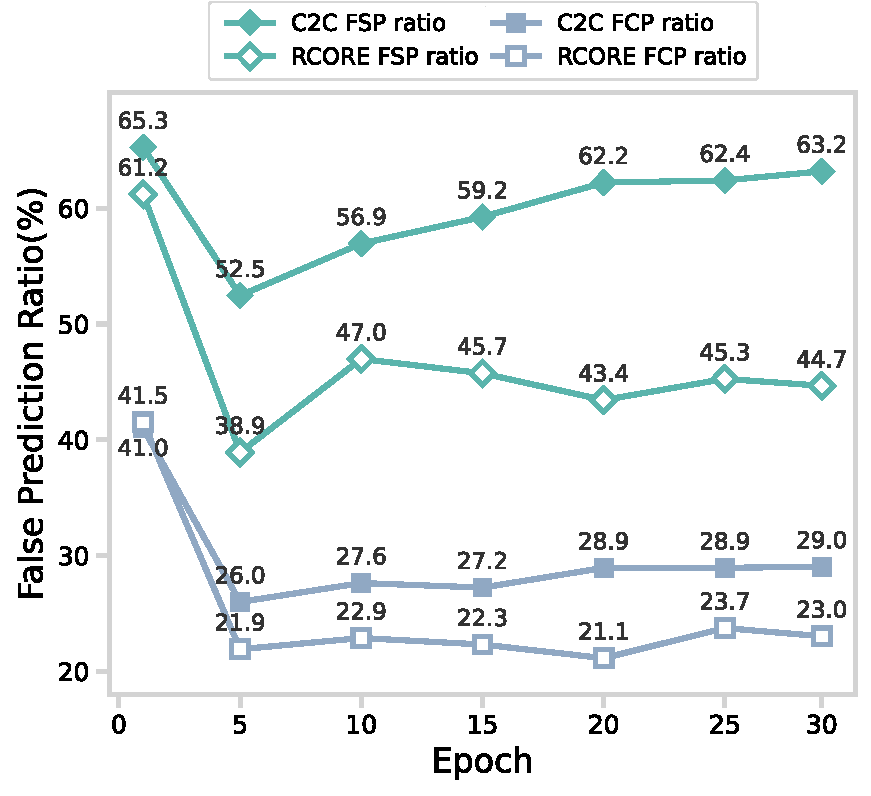
\includegraphics[width=\linewidth]{figure/src/validation/validation_fsp_curve.pdf}
\\
\scriptsize{\hspace{.5cm}(a)}
} 
\mpage{0.27}{
\centering    
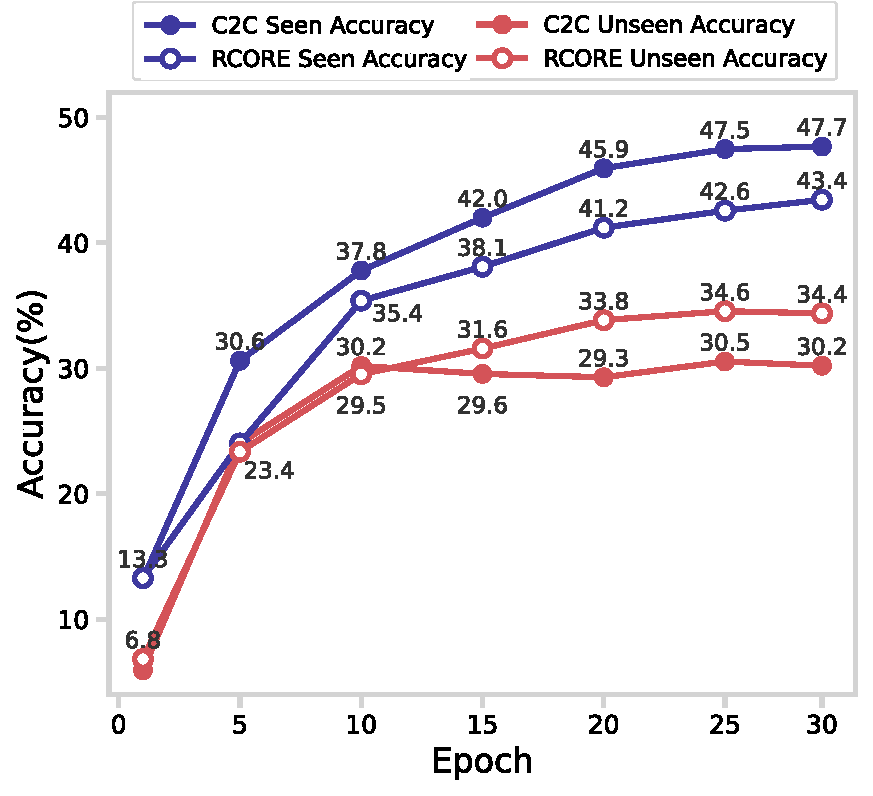
\includegraphics[width=\linewidth]{figure/src/validation/validation_acc_curve.pdf}
\\
\scriptsize{\hspace{.5cm}(b)}
}
\mpage{0.33}{
\centering    
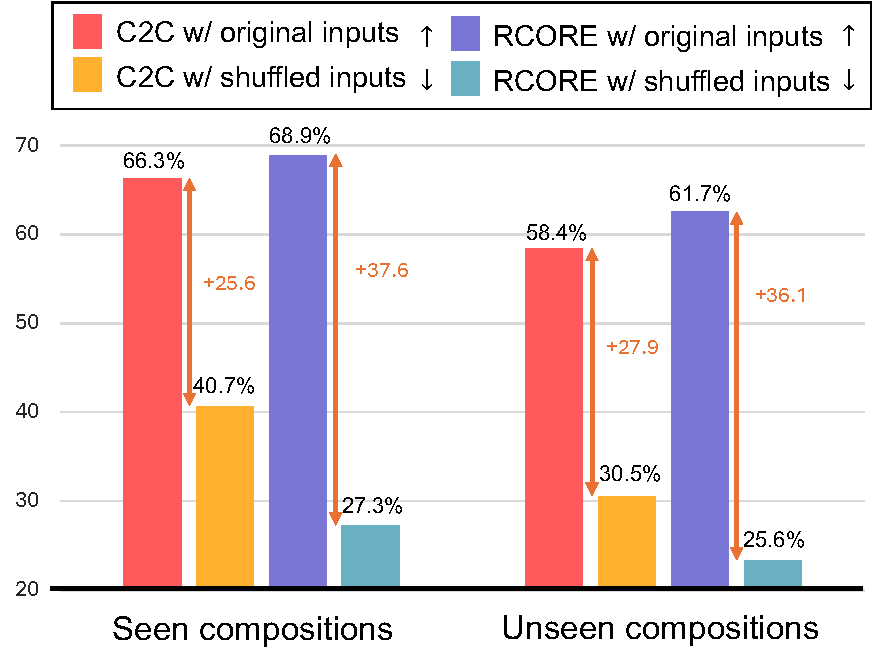
\includegraphics[width=\linewidth]{figure/src/validation/validation_shuffle_test.pdf}
\\
\scriptsize{\hspace{.5cm}(c)}
} 
\vspace{-1em}
\figcapmargin
\figcaption{Analysis on the effects of \ours{} on the Sth-com~\cite{li2024c2c} dataset}{
    (a) \ours{} suppresses the growth of FSP/FCP during training, unlike the baseline.
    (b) This reduces the seen–unseen gap and improves unseen composition accuracy.
    (c) On the temporal subset, \ours{} shows a larger drop under temporal shuffling, indicating stronger temporal dependence over static cues.
    Best viewed with zoom and color.
}
\label{fig:validation}
\end{figure}
